
\begin{figure}[ht]
  \centering
  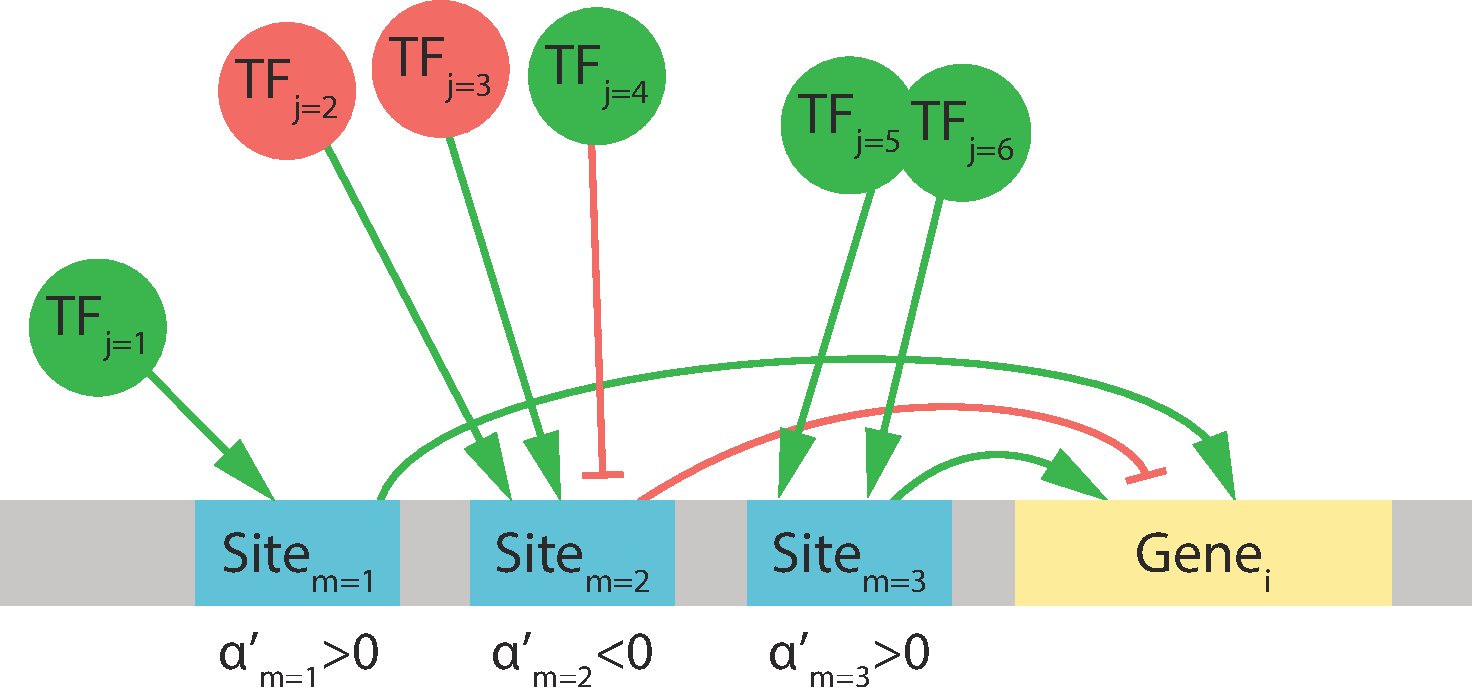
\includegraphics[width=\textwidth]{theory/fig/GeneWeaverRegulation.pdf}
  \caption{\textbf{Gene regulation model in GeneNetWeaver.} Example of gene regulation used in GeneNetWeaver by $f$. 
%   For binding site $m=2$ there are three proteins competing to bind, for $m=3$ there are two proteins cooperating in binding to the site. 
%   Inhibition is in red and activation in green. 
%   TFs are colored red if they are an overall repressor of the gene or green if not. 
  $\alpha_m'$ is the effect of bound site $m$ on activation of gene $i$ relative to baseline activation. 
  }
  \label{fig:gnw_regulation}
\end{figure}


